\documentclass [12pt,letterpaper]{article}
\usepackage[margin=1.5in]{geometry}
\usepackage{graphicx, lscape, url}

\setlength\parindent{0pt}

\begin{document}
 
% Titlepage
\thispagestyle{empty}
\begin{center}
    \centering
% University logo
    
\includegraphics[width=0.3\linewidth]{images/nottingham-logo.png}
    \vspace{0.1cm}
    {\Large \\University of Nottingham\par}
    {\Large Department of Computer Science\par}
    \vspace{3cm}
% Project title
    {\Large COMP3003 - Interim Report\par}
    \vspace{0.5cm}
    {\Large A Cross-platform Networking Configuration \& Auditing Mobile Application\par}
    \vspace{2.5cm}
% Author Name
    {\Large Jozef W. Sieniawski\par}
    {\small Computer Science BSc. \par}
    {\small 20296126 $|$ psyjs25@nottingham.ac.uk\par}
    \vspace{1cm}
% Supervisor
    {\normalsize Supervisor: Proff. Chris Greenhalgh\par}
    \vspace{3cm}
% Date
    {\Large September 2022}
\end{center}

% Table of contents
\pagebreak
\tableofcontents
\pagebreak

% Add spacing between paragraphs
\setlength{\parskip}{2ex}

% Introduction
\section{Introduction}
\label{sec:introduction}
\subsection{Background}
\label{sec:background}
\subsection{Aims}
\label{sec:aims}
\subsection{Objectives}
\label{sec:objectives}
\subsection{Scope}
\label{sec:scope}


\section{Motivation}
With the work for the Research Support Team in the School of Computer Science at Nottingham, one of the primary responsibilities revolves around server spaces. This involves the installation and configuration of new servers, as well as the maintenance of existing hardware. When we were faced with the task of migrating servers to a new location, the problem of understanding the configuration of the existing servers arose. There lacked a consistent documentation format that could be used to replicate the configuration of a server in a new location.

With a larger project in mind, where understanding the configuration of many servers was essential, the idea of this project was born; To create a tool that will allow for cable configuration of server hardware to be easily digitised, visualised, queried and updated.

Whilst alternatives exist, they are typically a segment of a far larger suite of tools, which are usually not necessary for small/medium sized server spaces. Naturally, cable configurations can be difficult to understand and work with even in these smaller spaces. This also brought forward the second aspect of the project, to also be an investigation into the user experience and interface design of the tool. To ensure that the tool is easy to use and can be understood by a wide range of users.

Further, the project will be open source, and will be available for use by the wider community of server administrators. This will allow for the human Computer interaction findings that have been implemented to be used in similar applications. Additionally, the tool will be utilising and integrating with Netbox, an open-source tool for managing network infrastructure. This will act as the backing database for the tool and will allow for the tool to be used in a wider context of server management.

The Research Support Team will act as a prime example of the target audience. The project aims to discover the needs of a wider range of small and medium sized enterprises (SME) who run and maintain their own server spaces. As mentioned previously, there are not many similar alternatives to the project as these SME's usually pose a unique server environment. These spaces can be cramped, poorly lit and hard to navigate.

This is another reason that typical solutions cannot usually apply to these spaces, as they are often designed for large data centres, where laptops can be used easily to use software in situ. A tool that can be used on a mobile device in these less-than-ideal conditions is something worth investigating. A perfect example of this is the server space in the School of Computer Science seen in the image below. Before upgrades, the space was poorly lit and is, still relatively cramped. It’s not particularly feasible to use a laptop in this space comfortably. The current layout of servers and hardware makes tracking cables completely impracticable.

\begin{figure}
    \centering
\begin{minipage}{.48\linewidth}
    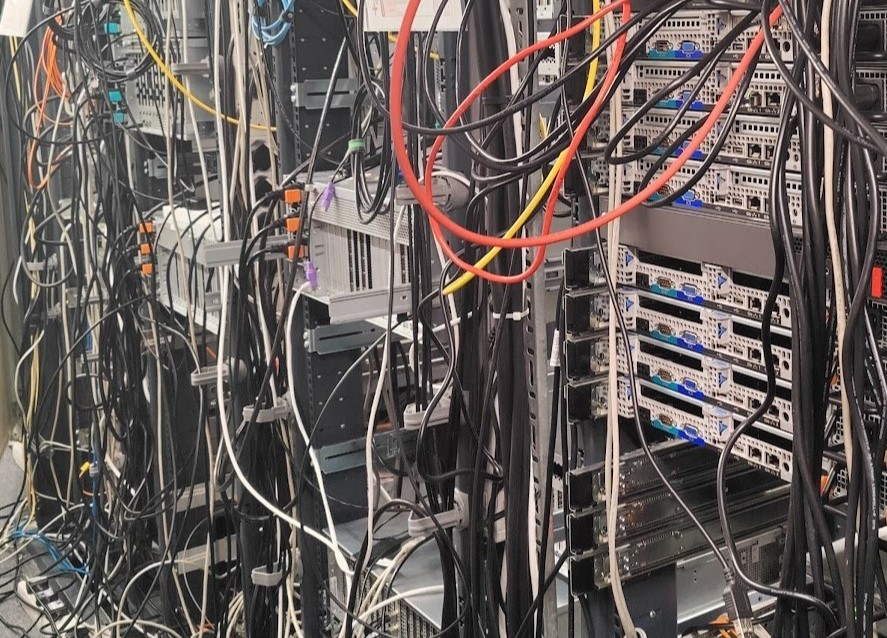
\includegraphics[width=\linewidth]{images/server_racks.jpg}
    \caption{Non-ideal server space}
    \label{"fig: Non-ideal server space"}
\end{minipage}
\hfill
\begin{minipage}{.48\linewidth}
    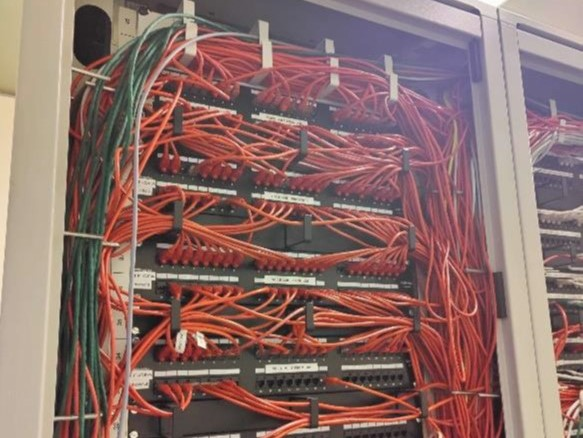
\includegraphics[width=\linewidth]{images/server_racks_clean.jpg}
    \caption{More ideal and realistic server space}
    \label{img2}
\end{minipage}
\end{figure}

Cum


\section{Related Work}

\section{Description of the Work}

\section{Methodology}

\section{Design}

\section{Implementation}

\section{Progress}

\section{Contributions and Reflections}


% Bibliography
\pagebreak
\bibliographystyle{ieeetr}
\bibliography{citation} 
% Document End
\end{document}